% Modified 31 Oct 2005:  Conditioning fallacy alluded to.
% This chapter has been modified on 6-4-05.
% There are two \choice
\pagestyle{headings}
\chapter{Combinatorics} \label{chp 2}
\thispagestyle{fancy}

\subsection*{Introduction: Traversing a Grid}
Consider a large city laid out in rectangular blocks, and a pedestrian who's walking to his workplace, ten blocks north and ten blocks east of his house. Our pedestrian won't waste his time by ever moving west or south; he has a schedule to keep. How many distinct paths are there from his house to his workplace?

\begin{center}
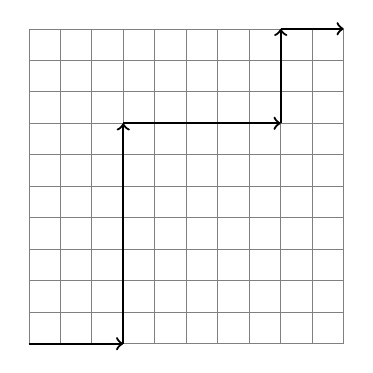
\begin{tikzpicture}[scale=0.4]
\draw[step=1cm,gray,very thin] (0,0) grid (10,10);
\draw[thick, ->] (0,0) -- (3,0);
\draw[thick, ->] (3,0) -- (3,7);
\draw[thick, ->] (3,7) -- (8,7);
\draw[thick, ->] (8,7) -- (8,10);
\draw[thick, ->] (8,10) -- (10,10);
\end{tikzpicture}
\end{center}
\par
At first glance, he has two options at each intersection he reaches, north or east, but eventually he'll have moved ten blocks in one of those two cardinal directions, and from that point on his decision will be forced. Unfortunately, the number of steps he takes until his options run out is not constant. Some paths will `hit the wall' sooner than others.
\par
Combinatorics is the field of mathematics concerned with counting problems like this one. These questions are often simple to state, and can have beautifully clever solutions. As we've done with probability theory, we'll develop some general principles which, when carefully applied, provide a basis for building solutions to many counting problems.
\newpage

\section{Permutations} \label{sec 2.1}

Suppose you order onion rings and a soda at a fast food restaurant. There are two options for the size of the onion rings ($S$/$L$) while there are three options for the size of the soda ($S$/$M$/$L$).
\par
Since there are two options for the size of the onion rings, and three options for the size of the soda, you have a total of six possible choices when you order both items. These are enumerated below, the first letter in each ordered pair denoting the size of the onion rings, and the second letter the size of the soda.
$$(S,S)\ \ (S,M)\ \ (S,L)\ \ (L,S)\ \ (L,M)\ \ (L,L)$$
\indent If there's only enough change in your pocket to pay for a single item (any size), then you have the five options given below.
$$(S, \, - \, )\ \ (L, \, - \, )\ \ (\, - \, , S) \ \ (\, - \, , M) \ \ (\, - \, , L)$$
\par
\begin{prop}(Fundamental Counting Principle) \label{FundamentalCountingPrinciple}\index{Fundamental Counting Principle} In a sequence of $k$ choices, if the first choice can be made in $n_1$ ways, the second choice can be made in $n_2$ ways, and so on, the number of ways of making all choices is the product $n_1 n_2 \,\cdots\, n_k$, while the number of ways of selecting one of the choices and making it is the sum $n_1 + n_2 + \,\dots\, + n_k$.
\end{prop}
\begin{examp}
How many ways are there to select three students to be class representatives in three different classes, one with twenty students and two with thirty?
\par
\noindent There are three choices to be made, choosing a representative for each of the three classes, and since we must make all three choices, the number of ways this can be done is $20 \cdot 30 \cdot 30 = 18\,000$.\end{examp}
\begin{examp}
How many four letter sequences can be made with only the first four letters of the alphabet?
\par
\noindent We can imagine filling in four blank spaces with letters, and write in each blank space the number of choices we have for the letter that gets placed there. If we allow repetition, then the number of sequences is $\underline{4} \cdot \underline{4} \cdot \underline{4} \cdot \underline{4} = 256$.
\par
\noindent If each space must be filled with a distinct letter, then initially there are four choices for the first letter, but after making that choice, there are three remaining for the second letter, and so on. In total then, the number of sequences with distinct letters is $\underline{4} \cdot \underline{3} \cdot \underline{2} \cdot \underline{1} = 24$. 
\par
\noindent This second result is the number of ways of rearranging the four letters $ABCD$, and counting rearrangements is something we'll do frequently, so it's convenient to make some notation.
\end{examp}
\par
\begin{defn}\index{Factorial}
Given $n \in \mathbb{N}$, the factorial of $n$, denoted $n!$, is the number of ways of arranging $n$ distinct objects in a line, and is defined by
$$n! = n \cdot (n-1) \cdot (n-2) \cdot \, \cdots \, \cdot 2 \cdot 1$$
\end{defn}
\begin{rmk} Though the interpretation of the factorial as counting arrangements no longer applies, we define $0!=1$ for convenience.
\end{rmk}
\par Factorials have some very nice algebraic properties that make them easy to work with, in particular, ratios of factorials can be simplified easily.
\eqnsgap{\frac{8!}{6!} = \frac{8 \cdot 7 \cdot 6 \cdot 5 \cdot 4 \cdot 3 \cdot 2 \cdot 1}{6 \cdot 5 \cdot 4 \cdot 3 \cdot 2 \cdot 1}= \frac{8 \cdot 7 \cdot \cancel{6} \cdot \cancel{5} \cdot \cancel{4} \cdot \cancel{3} \cdot \cancel{2} \cdot \cancel{1}}{\cancel{6} \cdot \cancel{5} \cdot \cancel{4} \cdot \cancel{3} \cdot \cancel{2} \cdot \cancel{1}} = 56}
\par
\begin{examp}
How many ways are there to choose three students from a class of twenty and arrange them in a line?
\par
\noindent We can use the same approach as in the last example. We're filling in three blanks, we have twenty options to choose from, and repeats are not permitted. Thus, there are $\underline{20} \cdot \underline{19} \cdot \underline{18} = 6\,840$ ways to do it. 
\par
\noindent The notation $^{20}P_3$ is used to refer to the number of ways of selecting $3$ objects from a set of $20$ distinct options and ordering them. Thus, we have $^{20}P_3 = 6\,840$.
\end{examp}
\par
\begin{definition}\label{permutationdefinition}\index{Permutations}
If an ordered list of $r$ distinct objects is selected from a set of $n$ objects, the result is called an $r$-permutation. The number of $r$-permutations of $n$ objects, denoted by $^{n}P_r$, is given by
\eqnsgap{\boxed{^nP_r = n \cdot (n-1) \cdot \, \cdots \, \cdot (n-r+1) = \frac{n!}{(n-r)!}}}
\end{definition}
\par
\begin{examp}
How many ways there there to create a sequence of five letters with no repetitions using any of the 26 letters of the alphabet?
\par
\noindent Taking $5$ letters from a set of $26$ and arranging them, the number of options is
$$^{26}P_5 = \frac{26!}{(26-5)!} = \frac{26!}{21!} = 26 \cdot 25 \cdot 24 \cdot 23 \cdot 22 = 7\,893\,600$$
\end{examp}

\subsection*{Permutations with Identical Objects}
\par
What if some objects are indistinguishable? If this is the case, there are fewer possibilities. For example, how many arrangements of the string $AAAB$ are there? We just have to decide which of the four possible positions we'll place the $B$ into, and then $A$s go everywhere else, so there are only four distinct arrangements.

Now suppose that we number the three $A$s. How many rearrangements of the string $A_1A_2A_3B$ are there? Since the four letters are now distinguishable, there are $4! = 24$. Let's write these out, grouping together in columns all strings that will be identical after the labels on the $A$s are removed.
\begin{center}
\begin{tabular}{cccc}
$A_1A_2A_3B$ & $A_1A_2BA_3$ & $A_1BA_2A_3$ & $BA_1A_2A_3$ \\
$A_1A_3A_2B$ & $A_1A_3BA_2$ & $A_1BA_3A_2$ & $BA_1A_3A_2$ \\
$A_2A_1A_3B$ & $A_2A_1BA_3$ & $A_2BA_1A_3$ & $BA_2A_1A_3$ \\
$A_2A_3A_1B$ & $A_2A_3BA_1$ & $A_2BA_3A_1$ & $BA_2A_3A_1$ \\
$A_3A_1A_2B$ & $A_3A_1BA_2$ & $A_3BA_1A_2$ & $BA_3A_1A_2$ \\
$A_3A_2A_1B$ & $A_3A_2B_1A$ & $A_3BA_2A_1$ & $BA_3A_2A_1$ \\
\end{tabular}
\end{center}
Notice that rearranging the labels will result in a string which is identical once the labels are removed. This means if we list all possible arrangements of the \emx{labeled strings}, each possible \emx{unlabeled string} will appear $k!$ times, where $k$ is the number of labels. In this case, each distinct unlabeled string appears $3! = 6$ times.
\par
The key point is that we can count the number of unlabeled strings by dividing the number of labeled strings by the number of ways of rearranging the labels, in this case, $4! / 3! = 4$. The same principle applies if there are many different kinds of indistinguishable objects.
\par
\begin{prop}\index{Mississippi Formula} (Mississippi Formula) The number of ways of rearranging $n$ objects, with indistinguishable groups of sizes $k_1, k_2, \dots\, ,k_m$, is given by
\eqnsgap{\boxed{\frac{n!}{k_{1}! \cdot k_{2}! \cdot \, \cdots \, \cdot k_{m}!}}}
\end{prop}
\par
\begin{examp}
How many arrangements of the letters in MISSISSIPPI are there?
\par
\noindent There are eleven letters in total, with identical groups of size 4 (the I's), 4 (the S's), and 2 (the P's). Therefore, the number of arrangements is
\eqnsbiggap{\frac{11!}{4! \cdot 4! \cdot 2!} = \frac{11 \cdot 10 \cdot 9 \cdot {8} \cdot 7 \cdot {6} \cdot 5 \cdot {4} \cdot {3} \cdot {2} \cdot 1}{{4} \cdot {3} \cdot {2} \cdot 1 \cdot {4} \cdot {3} \cdot {2} \cdot 1 \cdot {2} \cdot 1} = 11 \cdot 10 \cdot 9 \cdot 7 \cdot 5 = 34\,650.}
\end{examp}
\begin{examp}
An urn contains four green and five red marbles, which are removed one at a time. How many different ways are there to empty the urn?
\par
\noindent In this case, we are rearranging nine objects, each arrangement corresponds to a possible order in which they might appear when removed from the urn. There are identical groups of size 4 (the green marbles), and 5 (the red marbles). Therefore, the number of arrangements is
\eqnsbiggap{\frac{9!}{4! \cdot 5!} = \frac{9 \cdot {8} \cdot 7 \cdot {6} \cdot 5 \cdot {4} \cdot {3} \cdot {2} \cdot 1}{{4} \cdot {3} \cdot {2} \cdot 1 \cdot {5} \cdot {4} \cdot {3} \cdot {2} \cdot 1} = 9 \cdot 2 \cdot 7 = 126.}
\end{examp}

\section{Combinations}\label{sec 2.2}

Suppose now that we are interested in the number of ways that a subset of $r$ objects can be selected from a larger set of $n$ distinct objects. The order in which the selections are made doesn't matter, we're only concerned with which objects are selected.
\par
Consider how many ways there are to select three children from a family with five. To do this, we can imagine lining up the children any fixed order, let's say by age. We can now specify which children are chosen using a string such as $YYNYN$, which would indicate we chose the first two children in the line as well as the fourth. In fact, every distinct five letter string made up of $Y$s and $N$s which has exactly three $Y$s will represent a different choice of three children, and every choice of three children determines such a string.
\par
Now we can use the Mississippi formula to count the number of different choices by counting strings. Each string is a rearrangement of five objects with identical groups of sizes three and two, hence there are $\frac{5!}{3!2!} = 5 \cdot 2 = 10$ possibilities.
\par
The general principle is that once the elements of a set have been lined up in some arbitrary order, each subset is given by an \emph{ordered} list of $Y$'s and $N$'s, where $Y$ denotes membership in the subset, and $N$ denotes non-membership. We can count the number of ordered lists of $Y$'s and $N$'s by using the MISSISSIPPI formula.
\begin{defn}\index{Combinations}\label{combinationdefinition}
If a subset of $r$ objects is selected from a set of $n$ objects, the result is called an $r$-combination. The number of $r$-combinations, denoted $^nC_r$, or more commonly $\binom{n}{r}$, is given by
\eqnsgap{\boxed{^nC_r = \binom{n}{r} = \frac{n!}{r!(n-r)!}}}
\end{defn}
\begin{rmk}
Note the distinction between $^nP_r$ and $^nC_r$. The former counts the number of ways of selecting $r$ objects \emx{and arranging them}, while the latter is the number of selections possible when \emx{any rearrangement is regarded as the same outcome}.
\end{rmk}
\begin{examp}
In Lotto 6/49, if you purchase a ticket you choose 6 distinct numbers between 1 and 49. The ticket wins if its numbers match 6 distinct numbers between 1 and 49 which are randomly drawn, regardless of the order they are drawn in. How many different tickets would you need to buy to guarantee a win?
\par
\noindent Since the order of the numbers on the ticket is irrelevant, the number of different tickets available is $\binom{49}{6} = \frac{49!}{6!43!} = 13\,983\,816$, so this is the minimum number you would need to purchase to be sure one will win.
\end{examp}
\begin{examp}
How many ways are there to choose a president, a treasurer, and an organizing committee of three from a group of 25 people? Assume no person can hold more than one position.
\par
\noindent There are 25 choices for president, then 24 for treasurer, then $\binom{23}{3}$ for the organizing committee. Note that when choosing the organizing committee, the order in which members are chosen is irrelevant. The committee consisting of Alice, Bob, and Chelsea and the committee consisting of Chelsea, Alice, and Bob are the same.
\par
\noindent Since we must make all three choices, by the fundamental counting principle the number of possibilities is
\eqns{25 \cdot 24 \cdot \binom{23}{3} = 1\,062\,600.}
\par
\noindent Notice that we could just as well have proceeded in the opposite order in our analysis, that is, first chosen the organizing committee, then the treasurer, then the president, and still obtained
\eqnsgap{\binom{25}{3} \cdot 22 \cdot 21 = 1\,062\,600.}
\end{examp}
\begin{examp}How many ways are there to divide a group of eight people into a team of three and a team of five?
\par
\noindent To create a team of three and a team of five, we choose three individuals for the team of three, then the five remaining make up the team of five.
$$\binom{8}{3}\binom{5}{5} = 56$$
\end{examp}
\begin{examp}How many ways are there to divide a group of eight people into two teams of four?
\par
\noindent To create two teams of four, we choose four for the first team, and those that remain make up another team of four. We have to be very careful though. In the example above the two teams were distinguishable, but here they are not. 
\par
\noindent If we select A, B, C, and D for the first team and E, F, G, and H for the second, this results in the outcome as selecting E, F, G, and H for the first team and A, B, C, and D for the second. The teams are indistinguishable, so every outcome has been double counted! Thus, we need to divide out by the number of rearrangements of the teams.
$$\frac{\binom{8}{4}\binom{4}{4}}{2!} = 35$$
\par
\noindent Notice that if the two teams were distinguishable, for example, if we divide eight people into a marketing team and an administrative team with four people on each team, there would be $\binom{8}{4}\binom{4}{4} = 70$ ways.
\end{examp}

\subsection*{Poker Hand Probabilities}

In many variations of the gambling game poker, five cards are drawn from a shuffled deck to form a hand. The order of these cards is irrelevant, each player may freely rearrange his or her hand. We can use the counting techniques we've developed to compute the probabilities of drawing various hands.

\begin{examp}What is the probability of drawing a full house? In this hand, three of the five cards share a rank, and the remaining two also share a rank, for example, the cards could be $7 \spadesuit \, 7\heartsuit \, 7 \clubsuit \, Q \diamondsuit \, Q \heartsuit$.
\par
\noindent There are 13 possible ranks for the group of three cards and we must choose one. Once that's done, there is a pool of 12 remaining ranks for the other two, from which we must choose one. Thus, to fill in the ranks, we have $\binom{13}{1}\binom{12}{1}$ possibilities. If we choose, for example, $7$ for the group of three and $Q$ for the remaining two, we've determined the ranks as shown below.

\vspace{-1em}
\begin{center}
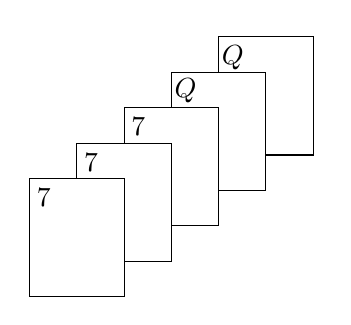
\begin{tikzpicture}[scale=0.6]
\draw (-2,-1.5) rectangle (0,1);
\draw (-1,1) node {} -- (-1,1.75) node {} -- (1,1.75) node {} -- (1,-0.75) node {} -- (0,-0.75) node {};
\draw (0,1.75) node {} -- (0,2.5) node {} -- (2,2.5) node {} -- (2,0) node {} -- (1,0) node {};
\draw (1,2.5) node {} -- (1,3.25) node {} -- (3,3.25) node {} -- (3,0.75) node {} -- (2,0.75) node {};
\draw (2,3.25) node {} -- (2,4) node {} -- (4,4) node {} -- (4,1.5) node {} -- (3,1.5) node {};
\node at (-1.7, 0.6) {$7$};
\node at (-0.7, 1.35) {$7$};
\node at (0.3, 2.1) {$7$};
\node at (1.3, 2.85) {$Q$};
\node at (2.3, 3.55) {$Q$};
\end{tikzpicture}
\end{center}
\vspace{-1em}

\noindent Note that if we instead choose $Q$ for the group of three and $7$ for the remaining two, we would produce a different hand, which has three queens and two sevens. This is good. We want distinct sequences of choices to produce distinct hands. If not, we would be double counting certain hands.
\par
\noindent To determine the suits, notice that we have four choices for each card, but within each group of identical ranks, suits cannot be repeated (there is only one 7 of hearts in a deck), and order does not matter since we can freely reorder the hand. Thus, there are $\binom{4}{3}$ options for the suits in the group of three cards of equal rank, and $\binom{4}{2}$ options for the suits in the group of two. Since both choices need to be made, we have a total of $\binom{4}{3}\binom{4}{2}$ options when determining the suits. After filling in the suits, we have completely determined the hand.

\vspace{-1em}
\begin{center}
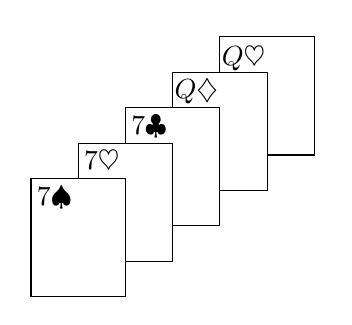
\begin{tikzpicture}[scale=0.6]
\draw (-2,-1.5) rectangle (0,1);
\draw (-1,1) node {} -- (-1,1.75) node {} -- (1,1.75) node {} -- (1,-0.75) node {} -- (0,-0.75) node {};
\draw (0,1.75) node {} -- (0,2.5) node {} -- (2,2.5) node {} -- (2,0) node {} -- (1,0) node {};
\draw (1,2.5) node {} -- (1,3.25) node {} -- (3,3.25) node {} -- (3,0.75) node {} -- (2,0.75) node {};
\draw (2,3.25) node {} -- (2,4) node {} -- (4,4) node {} -- (4,1.5) node {} -- (3,1.5) node {};
\node at (-1.5, 0.6) {$7\spadesuit$};
\node at (-0.5, 1.35) {$7\heartsuit$};
\node at (0.5, 2.1) {$7\clubsuit$};
\node at (1.5, 2.85) {$Q\diamondsuit$};
\node at (2.5, 3.55) {$Q\heartsuit$};
\end{tikzpicture}
\end{center}
\vspace{-1em}

\noindent Thus, there are $\binom{13}{1}\binom{12}{1}\binom{4}{3}\binom{4}{2}$ different full houses. Since there are $\binom{52}{5}$ possible five card subsets of a standard deck, and each is equally likely to be drawn if we suppose the deck is well shuffled, the probability of a full house is
$$\frac{\binom{13}{1}\binom{12}{1}\binom{4}{3}\binom{4}{2}}{\binom{52}{5}} = \frac{3\,744}{2\,598\,960} \simeq 0.14 \%.$$
\end{examp}
\begin{examp}What is the probability of drawing a straight? In this hand, all five cards have consecutive ranks, for example, the three cards could be $7 \spadesuit \, 8\diamondsuit \, 9 \heartsuit \, 10 \heartsuit \, J \diamondsuit$. Note that $A$ plays the role of both the highest and lowest possible rank.
\par
\noindent Again, let's deal with the ranks first, and then the suits. In a straight, the card of lowest rank determines the ranks of all other cards. If the lowest ranked card is a $7$, then each rank between $7$ and $J$ will appear once in the hand, as shown below.

\vspace{-1em}
\begin{center}
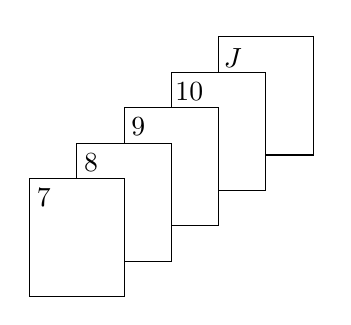
\begin{tikzpicture}[scale=0.6]
\draw (-2,-1.5) rectangle (0,1);
\draw (-1,1) node {} -- (-1,1.75) node {} -- (1,1.75) node {} -- (1,-0.75) node {} -- (0,-0.75) node {};
\draw (0,1.75) node {} -- (0,2.5) node {} -- (2,2.5) node {} -- (2,0) node {} -- (1,0) node {};
\draw (1,2.5) node {} -- (1,3.25) node {} -- (3,3.25) node {} -- (3,0.75) node {} -- (2,0.75) node {};
\draw (2,3.25) node {} -- (2,4) node {} -- (4,4) node {} -- (4,1.5) node {} -- (3,1.5) node {};
\node at (-1.7, 0.6) {$7$};
\node at (-0.7, 1.35) {$8$};
\node at (0.3, 2.1) {$9$};
\node at (1.38, 2.85) {$10$};
\node at (2.3, 3.55) {$J$};
\end{tikzpicture}
\end{center}
\vspace{-1em}

\noindent Since there are $10$ choices for the lowest ranked card, $A$ through $10$, and all the rest of the ranks are determined by that single card, there are $10$ possibilities. Now that the ranks are dealt with, what about the suits? Each card has a different rank, so suits can be repeated. There are $4$ choices for the suit of each card, and five cards, hence $4^5$ ways to assign suits by the fundamental counting rule.
\par
\noindent In total then, there are $10 \cdot 4^5$ possible straights, and thus the probability of drawing a straight is 
\eqns{\frac{10 \cdot 4^5}{\binom{52}{5}} = \frac{10\,240}{2\,598\,960} = 0.39\%.}
\par
\noindent Note that if all five cards also have the same suit, the hand is called a straight flush, so here we're including straight flushes (and royal flushes). If you'd like to correct for this, find the number of straight flushes (and royal flushes) and subtract it out.

\end{examp}



\section{The Binomial Theorem}

Consider the expression $(x+y)^n$, where $n \in \mathbb{N}$. Let's take the first few natural numbers for $n$ and expand this expression.

\vspace*{-0.5em}
\eqnsgap{(x+y)^1 &= x+y \\
\ \\
(x+y)^2 &= (x+y)(x+y) \\
&= xx + xy + yx + yy \\
&= x^2 + 2xy + y^2 \\
\ \\
(x+y)^3 &= (x+y)(x+y)(x+y) \\
&= xxx + xxy + xyx + xyy + yxx + yxy + yyx + yyy \\
&= x^3 + 3x^2y + 3xy^2 + y^3}
\par 
Once the exponent gets much larger, it becomes a real headache to go through the ordeal of expanding everything out. Wouldn't it be nice if there was a clever way to get straight to the result without having to go through all the work of expanding and collecting like terms?
\par
To expand $(x+y)(x+y)(x+y)$, we need to select a term from each of the three copies of the binomial expression $x+y$, either the left term, or the right term. We do this in each possible way one time to obtain the expansion. For instance, if we take the left term in the first two factors, and the right in the last,
\eqns{(\underline{x}+y)(\underline{x}+y)(x+\underline{y}) \ \rightarrow \ xxy.}
\par
In this way, we can associate strings of three $L$'s and $R$'s to terms in the expansion. Every such string will yield a distinct term in the expansion, simply by identifying $L$ with $x$ and $R$ with $y$.
\eqns{LLR \ \rightarrow \ (\underline{x}+y)(\underline{x}+y)(x+\underline{y}) \ \rightarrow \ xxy \\
RRR \ \rightarrow \ (x+\underline{y})(x+\underline{y})(x+\underline{y}) \ \rightarrow \ yyy \\
RLR \ \rightarrow \ (x+\underline{y})(\underline{x}+y)(x+\underline{y}) \ \rightarrow \ yxy}
\par
Consider the $3x^2y$ term in the expression $x^3 + 3x^2y + 3xy^2 + y^3$. It was obtained by adding up all terms in the expansion which had two $x$'s and one $y$. Each of these corresponds to a string with two $L$'s and one $R$. There are $\frac{3!}{2!1!} =3$ such strings by the Mississippi formula, and hence the coefficient of $x^2y$ after expanding $(x+y)^3$ and collecting like terms is $3$. The same idea applies in general.
\inbox{The coefficient of $x^ky^{n-k}$ in the expansion of $(x+y)^n$ is the same as the number of strings of $L$'s and $R$'s of length $n$ with exactly $k$ $L$'s, which is $\frac{n!}{k!(n-k)!} = \binom{n}{k}$ by the Mississippi formula.}
\par
This idea is often stated in the form of the theorem given below, and values of the form $\binom{n}{k}$ for some $n$ and $k$ are often referred to as binomial coefficients \index{Binomial Coefficients} because of this connection.
\par
\begin{thm}\index{Binomial Theorem}(Binomial Theorem) 
\eqnsgap{\boxed{(x+y)^n =\sum_{i=0}^{n} \binom{n}{i}x^{n-i}y^i = \binom{n}{0}x^n + \binom{n}{1}x^{n-1}y + \binom{n}{2}x^{n-2}y^2 + \cdots + \binom{n}{n}y^n}}
\end{thm}
\par
\rmk The first and last coefficients in the expansion are both one. This provides some motivation for defining $0! = 1$; it makes $\binom{n}{0}$ and $\binom{n}{n}$ both defined and equal to one, so the binomial theorem is simpler to state.
\begin{examp}
What is the last digit of the number $109^{2717}$?
\par
\noindent This number is much too large to actually write down digit by digit, but with clever use of the binomial theorem, we can determine the last digit without knowing any of the others. Notice that $109^{2717} = (110 - 1)^{2717}$, and by the binomial theorem,
\eqns{(110-1)^{2717} = \binom{2717}{0}110^{2717} + \binom{2717}{1}110^{2716} \cdot (-1)^1 +\cdots+ \binom{2717}{2717}(-1)^{2717}}
\par
\noindent Each term is a product of integers, and $110$ is a multiple of ten, hence so is $110^k$ for any integer $k$. Therefore, every term in the expansion is a multiple of ten except the last. This final term is $(-1)^{2717} = -1$. Therefore, $109^{2717}$ is one less than a multiple of ten, hence its last digit is a 9.
\par
\noindent
This argument can be generalized considerably. Take a power of any number, write the base as a sum or difference of a multiple of ten and a single digit number, then use the binomial theorem. If you can compute the last digit of the last term of the expansion, you'll know the last digit of the number in question.
\end{examp}

\subsection*{Pascal's Triangle}

\begin{center}
\begin{tabular}{c}
1 \\
1 \ \ \ 1 \\
1 \ \ \ 2 \ \ \ 1 \\
1 \ \ \ 3 \ \ \ 3  \ \ \ 1 \\
1 \ \ \ 4 \ \ \ 6 \ \ \ 4  \ \ \ 1 \\
1 \ \ \ 5 \, \  10 \ \ 10  \, \ 5  \ \ \ 1 \\
1 \ \ \ 6 \, \ 15 \ \ 20 \ \  15 \, \ 6 \ \ \ 1 \\
1 \ \ \ 7 \, \ 21 \ \ 35 \ \ 35  \ \  21 \, \ 7 \ \ \ 1 \\
\vdots
\end{tabular}
\end{center}

This unending arrangement of numbers is commonly known as Pascal's triangle, in honour of Blaise Pascal, French mathematician and founding father of probability theory. Each row begins and ends with a one, while all interior entries are obtained by summing the two entries on the left and right in the row above. For instance, if we were to write the next row, 70 would appear in the center.
\par
Observe that the second, third, and fourth rows are exactly the coefficients that appeared in the expansions of $(x+y)^1$, $(x+y)^2$, and $(x+y)^3$. Could this be true in general? Why?
\par
Amazingly enough, it's true! The numbers that appear in the $(n+1)^{th}$ row of Pascal's triangle are exactly the coefficients in the expansion of $(x+y)^n$. This can be a neat shortcut when we apply the binomial theorem. To expand $(a+x)^6$, for example, write the first seven rows of Pascal's triangle. From the seventh row,
\eqns{(a+x)^6 = a^6 + 6a^5x + 15a^4x^2 + 20a^3x^3 + 15a^2x^4 + 6ax^5 + x^6.}
\par
To understand how this can be, let's play with Pascal's triangle a little. Consider a sequence of steps, starting from the top of the triangle, each step moving either down \& left, or down \& right. Let's call such a sequence of steps a path. Take, for example, the highlighted path below which ends in the sixth row.

\begin{center}
\begin{tabular}{c}
\textbf{1} \\
\textbf{1} \ \ \ 1 \\
1 \ \ \ \textbf{2} \ \ \ 1 \\
1 \ \ \ 3 \ \ \ \textbf{3}  \ \ \ 1 \\
1 \ \ \ 4 \ \ \ \textbf{6} \ \ \ 4  \ \ \ 1 \\
1 \ \ \ 5 \, \  \textbf{10} \ \ 10  \, \ 5  \ \ \ 1 \\
1 \ \ \ 6 \, \ 15 \ \ 20 \ \  15 \, \ 6 \ \ \ 1 \\
1 \ \ \ 7 \, \ 21 \ \ 35 \ \ 35  \ \  21 \, \ 7 \ \ \ 1 \\
\vdots
\end{tabular}
\end{center}

As it meanders down the triangle, this path moved left, then right, then right, then left, then left, so it can be denoted using the string LRRLL. In fact, every string of five $L$'s and $R$'s with three $L$'s describes a path which terminates in the same place. For instance, RLLLR gives the path highlighted below.

\begin{center}
\begin{tabular}{c}
\textbf{1} \\
1 \ \ \ \textbf{1} \\
1 \ \ \ \textbf{2} \ \ \ 1 \\
1 \ \ \ \textbf{3} \ \ \ 3  \ \ \ 1 \\
1 \ \ \ \textbf{4} \ \ \ 6 \ \ \ 4  \ \ \ 1 \\
1 \ \ \ 5 \, \ \textbf{10} \ \ 10  \, \ 5  \ \ \ 1 \\
1 \ \ \ 6 \, \ 15 \ \ 20 \ \  15 \, \ 6 \ \ \ 1 \\
1 \ \ \ 7 \, \ 21 \ \ 35 \ \ 35  \ \  21 \, \ 7 \ \ \ 1 \\
\vdots
\end{tabular}
\end{center}

We already discovered that the number of strings with five $L$'s and $R$'s containing exactly three $L$'s is $\binom{5}{3}= 10$, but how does this same number miraculously appear when instead of counting paths, we simply add the 4 and 6 in the row above?
\par
The key point is that \emx{every path which ends at a particular location is obtained either by adding an $R$ to a path which ended directly above and to the left, or by adding an $L$ to a path that ended directly above and to the right}. Thus, the number of paths that end at any given location is always the sum of the number of paths that end directly above and to the left and the number of paths that end directly above and to the right.

\begin{prop} The number appearing $k+1$ places across in row $n+1$ of Pascal's triangle is $\binom{n}{k}$, and furthermore, this number counts each of the following.
\vspace{-0.75em}
\begin{itemize}
\item Subsets containing $k$ objects taken from a collection of $n$ distinct objects.
\item The coefficient of $x^{n-k}y^k$ in the expansion of $(x+y)^n$.
\item Strings of $L$'s and $R$'s of length $n$ with exactly $k$ $L$'s. 
\item Paths through Pascal's triangle ending $k+1$ places across in row $n+1$.
\end{itemize}
\end{prop}

\par
The problem presented at the beginning of this chapter can be solved using the same idea of representing paths with strings and counting the number of strings.

\begin{examp}Consider a large city laid out in rectangular blocks, and a pedestrian who's walking to his workplace, ten blocks north and ten blocks east of his house. Our pedestrian won't waste his time by ever moving west or south; he has a schedule to keep. How many distinct paths are there from his house to his workplace?

\begin{center}
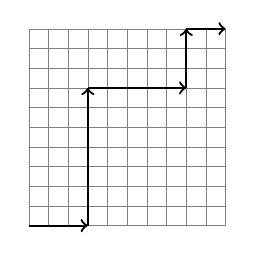
\begin{tikzpicture}[scale=0.25]
\draw[step=1cm,gray,very thin] (0,0) grid (10,10);
\draw[thick, ->] (0,0) -- (3,0);
\draw[thick, ->] (3,0) -- (3,7);
\draw[thick, ->] (3,7) -- (8,7);
\draw[thick, ->] (8,7) -- (8,10);
\draw[thick, ->] (8,10) -- (10,10);
\end{tikzpicture}
\end{center}

\par
\noindent Each path can be represented with a string of $E$'s and $N$'s, representing a sequence of movements one unit east ($E$), or one unit north ($N$). The path shown above, for example, corresponds to the string $EEENNNNNNNEEEEENNNEE$. Every path yields a string of $20$ $E$'s and $N$'s, exactly 10 of which are $E$'s. Therefore, the total number of possible paths is
\eqns{\binom{20}{10} = 184\,756.}

\end{examp}

\begin{comment}

\section{Partitions}

Suppose we have $7$ identical marbles and $3$ distinguishable boxes. How many ways are there to partition the marbles among the boxes?
\par
There's a really beautiful and simple way to solve this problem. We represent the seven marbles with seven identical stars. To partition the marbles among the boxes, we simply insert two bars. The diagram below, for example, represents a partition with one marble in the first box, two marbles in the second, and four marbles in the third.
$$*\,|**\,|****$$
To represent a partition where all marbles are in the first box, we can draw the following diagram.
$$*******\,|\,|$$
If all marbles are placed in the third box, we have the diagram below. Note that this is a different partition than the last, since the three boxes are distinguishable.
$$|\,|******\,*$$
\par
This idea, often called the stars \& bars \index{Stars \& Bars} method, was popularized in a book by William Feller \cite{Feller}. To count the number of partitions, we count the diagrams.
\par
Each diagram consists of $9$ symbols, $2$ of which are bars. Once the positions of the bars have been determined, all other positions must be filled in with stars. The order of the choices is not relevant, only which positions are chosen for the bars. Thus, there are $\binom{9}{2} = 36$ ways to partition the $7$ marbles among the $3$ boxes.

\begin{prop}\label{StarsAndBars} (Stars \& Bars) The number of ways of partitioning $n$ identical objects into $k$ distinguishable groups is 
\eqnsgap{\binom{n+k-1}{k-1}}
\end{prop}

\begin{examp} How many ordered triples $(x,y,z)$ of nonnegative whole numbers are solutions to the equation $x+y+z=15$?
\par
\noindent In this case, we can think of $15$ as the sum of $15$ ones, and partition these ones into three groups, one for each variable. The stars \& bars diagram below, for example, represents the partition $7+3+5$.
$$*******\,|***|****\,*$$
Thus, there are $\binom{17}{2} = 136$ ordered triples which sum to 15.
\end{examp}

\begin{examp} How many ordered triples $(x,y,z)$ of positive whole numbers are solutions to the equation $x+y+z=15$?
\par
\noindent Notice the difference. Zero is not a positive number, so we are not allowing empty groups. We would like to exclude partitions such as $7+9+0$.
$$*******\,|*********|$$
There is a very simple yet very clever idea we can use. Notice that if $x+y+z = 12$, then $(x+1)+(y+1)+(z+1) = 15$. Every ordered triple of nonnegative numbers which sums to 12 will yield a unique ordered triple of strictly positive numbers that sums to 15 after we add one to each variable. 
\par
\noindent In other words, we can imagine that before the partitioning, each variable already starts at one, so we partition the 12 remaining ones to end up with a sum of 15. Thus, there are $\binom{14}{2} = 91$ possibilities.
\end{examp}

\begin{examp} How many positive whole numbers under $10\,000$ have a digit sum of twelve? (For example, $7014$ has a digit sum of twelve since $7+0+1+4 = 12$)
\par
\noindent All such numbers have four or fewer digits, and if we allow digits to be zero, then we're simply partitioning twelve ones into four groups, one for each digit. As above, we can represent such a partition using stars \& bars. The number $3063$, for example, corresponds to the diagram below.
$$***\,|\,|******\,|**\,*$$
However, there is a problem. Some partitions will place more than 9 stars between two bars, and the largest possible digit is 9. We'll have to subtract these to come up with the correct count.
\par
\noindent Suppose that the first group (the leftmost) contains more than nine stars. We can generate all such diagrams by assuming ten stars have already been placed in the first group, then partitioning the rest freely. Since there are two stars left to partition using the three bars, there are a total of $\binom{5}{2}$ possibilities. 
\par
\noindent The same argument can be made for diagrams with more than nine stars in each of the four possible groups, hence there are total of $4 \cdot \binom{5}{2}$ partitions we need to subtract. Therefore, the number of positive whole numbers under 10\,000 whose digits sum to twelve is $\binom{15}{3} - 4\cdot\binom{5}{2} = 415$.
\end{examp}

\end{comment}

%Mention fcatalan numbers, generating functions, etc are very accessible and reference Art and craft oif problem ssoliving at end of section





